% Sostituisco i placeholder registrati con la specifica variabile per il documento corrente. Questa parte iniziale contiene intestazioni e templates.

% Modificare ad ogni modifica e documento
\newcommand{\documento}{\PdQ}
\newcommand{\nomedocumentofisico}{PianoDiQualifica 1\_0\_0.pdf}
\newcommand{\redazione}{\AN \\ & \DAN \\ & \DS}
\newcommand{\verifica}{\MC}
\newcommand{\versione}{1.0.0}
\newcommand{\approvazione}{\NS}
\newcommand{\uso}{Esterno}
\newcommand{\destinateTo}{\TV, \\ & \RC, \\ & \IS}
\newcommand{\datacreazione}{20 Dicembre 2016}
\newcommand{\datamodifica}{6 gennaio 2016}
\newcommand{\stato}{Approvato}

%Abilitazione indice delle tabelle e figure
\def\TABELLE{false}
\def\FIGURE{false}

%Inclusione di layout e variabili (Non modificare)
%Stile e dimensione del documento
\documentclass[a4paper,11pt]{article}

%Pacchetti da importare
\usepackage{ifthen}
\usepackage[italian]{babel}
\usepackage[utf8]{inputenc}
\usepackage[T1]{fontenc}
\usepackage{float}
\usepackage{chapterbib}
\usepackage{graphicx}
\usepackage[a4paper,top=2.5cm,bottom=2.5cm,left=2.5cm,right=2.5cm]{geometry}
\usepackage[colorlinks=true, urlcolor=black, citecolor=black, linkcolor=black]{hyperref}
\usepackage{booktabs}
\usepackage{fancyhdr}
\usepackage{totpages}
\usepackage{tabularx, array}
\usepackage{dcolumn}
\usepackage{epstopdf}
\usepackage{booktabs}
\usepackage{fancyhdr}
\usepackage{longtable}
\usepackage{calc}
\usepackage{datatool}
\usepackage[bottom]{footmisc}
\usepackage{listings}
\usepackage{textcomp}
\usepackage{titlesec}
\usepackage{rotating}
\usepackage{multirow}
\usepackage{placeins}
\usepackage{color}
\usepackage[table,usenames,dvipsnames]{xcolor}
\usepackage{hyperref}
\usepackage{makecell}
\usepackage{breakurl}
\usepackage{hyperref}
\usepackage{multirow}
\usepackage{xcolor,colortbl}
\usepackage{afterpage}



%Stile fancy per il documento (Header e footer)
\pagestyle{fancy}
%Rimuovo l'indentazione
\setlength{\parindent}{0pt}

%Imposto l'intestazione
\lhead{\Large{\progetto} \\ \footnotesize{\documento}}
%Linea sotto l'intestazione
\renewcommand{\headrulewidth}{0.4pt} 

%Footer
\lfoot{\textit{\gruppoLink}\\ \footnotesize{\email}}
%Footer con numero romano per le prime pagine
\rfoot{\thepage}
\cfoot{}
%Linea sopra il footer
\renewcommand{\footrulewidth}{0.4pt}   

%Imposta il livello degli elenchi 
\setcounter{secnumdepth}{7}
\setcounter{tocdepth}{7}

%Paragrafi impostati come una sezione
\titleformat{\paragraph}{\normalfont\normalsize\bfseries}{\theparagraph}{1em}{}
\titlespacing*{\paragraph}{0pt}{3.25ex plus 1ex minus .2ex}{1.5ex plus .2ex}

\titleformat{\subparagraph}{\normalfont\normalsize\bfseries}{\thesubparagraph}{1em}{}
\titlespacing*{\subparagraph}{0pt}{3.25ex plus 1ex minus .2ex}{1.5ex plus .2ex}

\makeatletter
\newcounter{subsubparagraph}[subparagraph]
\renewcommand\thesubsubparagraph{
  \thesubparagraph.\@arabic\c@subsubparagraph}
\newcommand\subsubparagraph{
  \@startsection{subsubparagraph}
    {6}
    {\parindent}
    {3.25ex \@plus 1ex \@minus .2ex}
    {0.75em}
    {\normalfont\normalsize\bfseries}}
\newcommand\l@subsubparagraph{\@dottedtocline{6}{10em}{5.5em}} 
\newcommand{\subsubparagraphmark}[1]{}
\makeatother

\makeatletter
\newcounter{subsubsubparagraph}[subsubparagraph]
\renewcommand\thesubsubsubparagraph{
  \thesubsubparagraph.\@arabic\c@subsubsubparagraph}
\newcommand\subsubsubparagraph{
  \@startsection{subsubsubparagraph}
    {7}
    {\parindent}
    {3.25ex \@plus 1ex \@minus .2ex}
    {0.75em}
    {\normalfont\normalsize\bfseries}}
\newcommand\l@subsubsubparagraph{\@dottedtocline{7}{10em}{6.5em}}
\newcommand{\subsubsubparagraphmark}[1]{}
\makeatother

%Variabili generali
\newcommand{\progetto}{API Market}
\newcommand{\gruppo}{NetBreak}
\newcommand{\gruppoLink}{\href{https://git.io/v1Rgz}{NetBreak}}
\newcommand{\email}{netbreakswe@gmail.com}

%Variabili riguardanti i documenti
\newcommand{\AdR}{Analisi dei Requisiti}
\newcommand{\NdP}{Norme di Progetto}
\newcommand{\PdP}{Piano di Progetto}
\newcommand{\SdF}{Studio di Fattibilità}
\newcommand{\PdQ}{Piano di Qualifica}
\newcommand{\VI}{Verbale Interno}
\newcommand{\VE}{Verbale Esterno}
\newcommand{\ST}{Specifica Tecnica}
\newcommand{\DDP}{Definizione di Prodotto}
\newcommand{\MU}{Manuale Utente}
\newcommand{\G}{Glossario}
\newcommand{\LdP}{Lettera di Presentazione}

%Variabili per i membri del gruppo
\newcommand{\AS}{Andrea Scalabrin}
\newcommand{\NS}{Nicolò Scapin}
\newcommand{\AN}{Alberto Nicolè}
\newcommand{\DS}{Davide Scarparo}
\newcommand{\DAN}{Dan Serbanoiu}
\newcommand{\MC}{Marco Casagrande}

%Ruoli di progetto
\newcommand{\RdP}{Responsabile di Progetto}
\newcommand{\Res}{Responsabile}
\newcommand{\Amm}{Amministratore}
\newcommand{\Ver}{Verificatore}
\newcommand{\Prog}{Progettista}
\newcommand{\Progr}{Programmatore}
\newcommand{\Ana}{Analista}
\newcommand{\RdPs}{Responsabili di Progetto}
\newcommand{\Ress}{Responsabile}
\newcommand{\Amms}{Amministratori}
\newcommand{\Vers}{Verificatori}
\newcommand{\Progs}{Progettisti}
\newcommand{\Progrs}{Programmatori}
\newcommand{\Anas}{Analisti}

%Professori e proponente
\newcommand{\TV}{Prof. Tullio Vardanega}
\newcommand{\RC}{Prof. Riccardo Cardin}
\newcommand{\IS}{ItalianaSoftware S.r.l.}
\newcommand{\proponente}{ItalianaSoftware S.r.l.}

\newcommand{\diaryEntry}[5]{#2 & \emph{#4} & #3 & #5 & #1\\ \hline}

%Comando per una nuova riga nella tabella del changelog
\newcommand{\specialcell}[2][c]{%
	\begin{tabular}[#1]{@{}c@{}}#2\end{tabular}}

\renewcommand*\sectionmark[1]{\markboth{#1}{}}
\renewcommand*\subsectionmark[1]{\markright{#1}}

%Variabili per la fase di lavoro
\newcommand{\AR}{Analisi dei Requisiti}
\newcommand{\PA}{Progettazione Architetturale}
\newcommand{\PD}{Progettazione Architetturale Dettagliata}
\newcommand{\CO}{Codifica}
\newcommand{\VV}{Verifica e Validazione}

%Variabili per le varie revisioni
\newcommand{\RR}{Revisione dei Requisiti}
\newcommand{\RP}{Revisione di Progettazione}
\newcommand{\RPMin}{Revisione di Progettazione Minima}
\newcommand{\RPMax}{Revisione di Progettazione Massima}
\newcommand{\RQ}{Revisione di Qualifica}
\newcommand{\RA}{Revisione di Accettazione}

\newcommand{\myincludegraphics}[2][]{%
	\setbox0=\hbox{\phantom{X}}%
	\vtop{
		\hbox{\phantom{X}}
		\vskip-\ht0
		\hbox{\includegraphics[#1]{#2}}}}

\renewcommand\footnoterule{\rule{\linewidth}{1pt}}

\newcommand{\nogloxy}[1]{#1} % comando da usare per evitare di metttere il mark del glossario
\newcommand{\gloxy}[1]{\emph{#1}$_G$}

\colorlet{punct}{red!60!black}
\definecolor{background}{HTML}{EEEEEE}
\definecolor{delim}{RGB}{20,105,176}
\colorlet{numb}{magenta!60!black}
\lstdefinelanguage{json}{
	basicstyle=\small\ttfamily,
	numbers=left,
	numberstyle=\scriptsize,
	stepnumber=1,
	numbersep=8pt,
	showstringspaces=false,
	breaklines=true,
	frame=lines,
	backgroundcolor=\color{background},
	literate=
	*{0}{{{\color{numb}0}}}{1}
	{1}{{{\color{numb}1}}}{1}
	{2}{{{\color{numb}2}}}{1}
	{3}{{{\color{numb}3}}}{1}
	{4}{{{\color{numb}4}}}{1}
	{5}{{{\color{numb}5}}}{1}
	{6}{{{\color{numb}6}}}{1}
	{7}{{{\color{numb}7}}}{1}
	{8}{{{\color{numb}8}}}{1}
	{9}{{{\color{numb}9}}}{1}
	{:}{{{\color{punct}{:}}}}{1}
	{,}{{{\color{punct}{,}}}}{1}
	{\{}{{{\color{delim}{\{}}}}{1}
	{\}}{{{\color{delim}{\}}}}}{1}
	{[}{{{\color{delim}{[}}}}{1}
	{]}{{{\color{delim}{]}}}}{1},
}
\lstset{language=json}
\lstset{literate=%
	{Ö}{{\"O}}1
	{Ä}{{\"A}}1
	{Ü}{{\"U}}1
	{é}{{\"s}}1
	{è}{{\"e}}1
	{à}{{\"a}}1
	{ö}{{\"o}}1
}

\newcommand{\impl}{\textcolor{Green}{Implementato}}
\newcommand{\implno}{\textcolor{Red}{Non Implementato}}
\newcommand\Tstrut{\rule{0pt}{3.2ex}}         % = `top' strut
\newcommand\Bstrut{\rule[-1.9ex]{0pt}{0pt}}   % = `bottom' strut
\definecolor{Gray}{gray}{0.85}
\usepackage[inline]{enumitem}

%Inclusione del changelog per il documento corrente
\newcommand{\modifiche}
{	
	Approvazione documento & \specialcell[t]{\DS\\\Res} & \specialcell[t]{2017-03-04\\2.0.0}
	\\
	\hline
	Verifica documento & \specialcell[t]{\MC\\\Ver} & \specialcell[t]{2017-03-03\\1.1.0}
	\\
	\hline
	Stesura sezione "Resoconto attività di verifica" & \specialcell[t]{\DS\\\Ana} & \specialcell[t]{2017-03-01\\1.0.4}
	\\
	\hline
	Nuova stesura sezione "Qualità di prodotto" & \specialcell[t]{\NS\\\Ana} & \specialcell[t]{2017-02-28\\1.0.3}
	\\
	\hline
	Nuova stesura sezione "Qualità di processo" & \specialcell[t]{\DS\\\Ana} & \specialcell[t]{2017-02-24\\1.0.2}
	\\
	\hline
	Ristrutturazione documento secondo suggerimenti del committente & \specialcell[t]{\DS\\\Ana} & \specialcell[t]{2017-02-23\\1.0.1}
	\\
	\hline
	Approvazione documento & \specialcell[t]{\NS\\\Res} & \specialcell[t]{2017-01-03\\1.0.0}
	\\
	\hline
	Effettuate modifiche secondo verifica & \specialcell[t]{\DS\\\Ana} & \specialcell[t]{2016-12-31\\0.1.1}
	\\
	\hline
	Verifica documento & \specialcell[t]{\MC\\\Ver} & \specialcell[t]{2016-12-29\\0.1.0}
	\\
	\hline
	Creata sezione "Qualità di prodotto" & \specialcell[t]{\DS\\\Ana} & \specialcell[t]{2016-12-28\\0.0.5}
	\\
	\hline
	Creata sezione "Qualità di processo" & \specialcell[t]{\DAN\\\Ana} & \specialcell[t]{2016-12-26\\0.0.4}
	\\
	\hline
	Creata sezione "Definizione obiettivi di qualità" & \specialcell[t]{\AN\\\Ana} & \specialcell[t]{2016-12-23\\0.0.3}
	\\
	\hline
	Creata introduzione & \specialcell[t]{\AN\\\Ana} & \specialcell[t]{2016-12-22\\0.0.2}
	\\
	\hline	
	Creato template documento & \specialcell[t]{\AS\\\Res} & \specialcell[t]{2016-12-20\\0.0.1}
	\\	
	
}

%Imposto la profondità degli indici
\setcounter{secnumdepth}{7}
\setcounter{tocdepth}{7}

\begin{document}

%Inclusione del template per la homepage (Non modificare)
%Importante: Non modificare questo template
%Modificare il documento principale per cambiare le parti

\begin{center}


%Spaziatura verticale

\vspace{4em}

%Intestazione con nome del gruppo
\begin{center} 
	\begin{Huge}
		\textbf{\fontsize{15mm}{20mm}\selectfont \gruppoLink} 
	\end{Huge}
\end{center}

\begin{center}
	\begin{Large}
		\vspace{0.3em}
		\textbf{Progetto \progetto}
	\end{Large}
\end{center}

%Inclusione del logo

\includegraphics[keepaspectratio = true,width=6cm]{../../Template/img/LogoNetbreak.png}

%Prima pagina senza intestazione né piè di pagina	
\thispagestyle{empty}

%Le informazioni del documento sono ancorate a fine pagina
\vfill

%Nome del documento
\begin{Huge} \textbf{\documento} \end{Huge}

%Tabella centrale
\begin{center}
\large\textbf{Informazioni sul documento} \\ \vspace{2em}
\small
\begin{tabular}{r l}
	\textbf{Nome del file} & \nomedocumentofisico \\
	\textbf{Data di creazione} & \datacreazione\\
	\textbf{Ultima modifica e versione} & \datamodifica\\ & Versione \versione\\
	\textbf{Stato} & \stato \\
	\textbf{Redatto da}	& \redazione\\
	\textbf{Verificato da}	& \verifica\\
	\textbf{Approvato da}	& \approvazione\\
	\textbf{Uso}  & \uso\\
	\textbf{Distribuzione} & \gruppo \\
	\textbf{Destinato a}  &  \destinateTo \\
\end{tabular}
\end{center}

\vspace{2em}

\normalsize
%Inclusione abstract
\textbf{Abstract\\} 


\end{center}
\clearpage


%Registro delle modifiche e indice (Non modificare)
\pagenumbering{Roman}
\newpage
% Non modificare - Pagina di Layout per il changelog
\begin{center}
	\Large{\textbf{Changelog}}
	\\\vspace{0.5cm}
	\normalsize
	\begin{tabularx}{\textwidth}{cXcc}
		\textbf{Versione} & \textbf{Descrizione} & \textbf{Autore e Ruolo} & \textbf{Data}
		\\\toprule
		\modifiche
		\bottomrule
	\end{tabularx}
\end{center}

%Inserisce il link all'indice
%\addcontentsline{toc}{section}{Indice}
\newpage
\tableofcontents
\clearpage 

%Se è stata impostata a true la variabile per la lista delle tabelle, la mostra
\ifthenelse{\equal{\TABELLE}{true}} 
{\listoftables \newpage}{}

%Se è stata impostata a true la variabile per la lista delle figure, la mostra
\ifthenelse{\equal{\FIGURE}{true}}
{\listoffigures \newpage}{}

%Da qui comincia la numerazione normale
\pagenumbering{arabic}

%Imposta il formato di visualizzazione
\rfoot{\thepage~di~\pageref{TotPages}}

%Inclusione delle varie sezioni di contenuto
%Introduzione e contenuti di ogni tipo


\newpage
\section{Introduzione}

\subsection{Scopo del documento}
Questo documento descrive le scelte e le strategie attuate per permettere di raggiungere determinati obiettivi di qualità misurabili. A questo scopo, sarà necessario un continuo processo di Verifica, orientato ad individuare e correggere errori ed eventuali sprechi di risorse.
Per conseguire dei risultati concreti, il processo di Verifica dovrà fornire dei dati quantificabili per poter valutare se gli obiettivi sono stati raggiunti o meno. Per facilitarne la valutazione, per ogni metrica sarannno indicati due range:
\begin{itemize}
	\item \textbf{Range accettazione:} rappresenta l'intervallo di valori minimi richiesti per il raggiungimento degli obiettivi di qualità definiti;
	\item \textbf{Range ottimale:} rappresenta l'intervallo di valori desiderati, entro cui dovrebbe collocarsi la misurazione. Nel caso in cui non si rientrasse in questo range, sarà necessario effettuare una verifica più accurata, al fine di individuarne le cause e poter applicare le dovute correzioni.
\end{itemize}

\subsection{Scopo del prodotto}
Lo scopo del prodotto è la realizzazione di un \textit{API Market\ped{G}} per l'acquisto e la vendita di \textit{microservizi\ped{G}}. Il sistema offrirà la possibilità di registrare nuove \textit{API\ped{G}} per la vendita, permetterà la consultazione e la ricerca di API ai potenziali acquirenti, gestendo i permessi di accesso ed utilizzo tramite creazione e controllo di relative \textit{API key\ped{G}}. Il sistema, oltre alla web app stessa, sarà corredato di un \textit{API Gateway\ped{G}} per la gestione delle richieste e il controllo delle chiavi, e fornirà funzionalità avanzate di statistiche per il gestore della piattaforma e per i fornitori dei microservizi.

\subsection{Riferimenti normativi}
\begin{itemize}
\item \textsc{NormeDiProgetto 3\_0\_0.pdf};
\item \textbf{Capitolato d’appalto C1:} APIM: An API Market Platform\\ \url{http://www.math.unipd.it/~tullio/IS-1/2016/Progetto/C1.pdf};
\end{itemize}

\subsection{Riferimenti informativi}
\begin{itemize}
	\item \textsc{PianoDiProgetto 3\_0\_0.pdf};
	\item \textbf{Slide del corso riguardo la qualità di prodotto}\\ \url{http://www.math.unipd.it/~tullio/IS-1/2016/Dispense/L10.pdf};
	\item \textbf{Slide del corso riguardo la qualità di processo}\\ \url{http://www.math.unipd.it/~tullio/IS-1/2016/Dispense/L11.pdf};
	\item \textbf{Standard ISO/IEC 12207:2008}\\ \url{https://www.iso.org/obp/ui/#iso:std:iso-iec:12207:ed-2:v1:en};
	\item \textbf{Standard ISO 9001}\\ \url{https://www.iso.org/iso-9001-quality-management.html};
	\item \textbf{Standard ISO/IEC 9126:2001}\\ \url{https://en.wikipedia.org/wiki/ISO/IEC_9126};
	\item \textbf{Standard ISO/IEC 15504}\\ \url{https://en.wikipedia.org/wiki/ISO/IEC_15504};
	\item \textbf{Indice Gulpease}\\ \url{https://it.wikipedia.org/wiki/Indice_Gulpease};	
\end{itemize}

\subsection{Glossario}
Per semplificare la consultazione e disambiguare alcune terminologie tecniche, le voci indicate con la lettera \textit{G} a pedice sono descritte approfonditamente nel documento \textsc{Glossario 3\_0\_0.pdf} e specificate solo alla prima occorrenza all'interno del suddetto documento.
\newpage
\section{Definizione obiettivi qualità}
	
	Prendendo come riferimento lo standard [ISO/IEC 9126] il team si impegna a
	garantire nel prodotto API Market le seguenti qualità:
	
	\subsection{Funzionalità}
		Per soddisfare questo obiettivo di qualità, il prodotto deve soddisfare i requisiti descritti nel documento \textsc{AnalisiDeiRequisiti1\_0\_0.pdf}.  
		
		\begin{itemize}
			\item \textbf{Misura: }quantità di requisiti mappati;
			\item \textbf{Metrica: }la sufficienza è definita dal numero di requisiti obbligatori. Ogni requisito secondario andrà ad aumentare la qualità del prodotto, ma la priorità dovrà essere data ai requisiti obbligatori;
			\item \textbf{Strumenti: }il sistema dovrà superare tutti i test previsti. Gli strumenti utilizzati sono descritti nel documento \textsc{NormeDiProgetto 1\_0\_0.pdf}.
			
		\end{itemize}
	
	\subsection{Affidabilità}
		Il sistema dovrà dimostrarsi il più possibile robusto e garantire, in modo particolare, la disponibilità del servizio di API gateway in percentuale più alta possibile. 
		
		\begin{itemize}
			\item \textbf{Misura: }l’unità di misura utilizzata sarà il numero di chiamate a microservizi andate a buon fine;
			\item \textbf{Metrica: }il limite di sufficienza riguarderà il numero di chiamate e il tempo che il sistema impiegherà per portarle a buon fine;
			\item \textbf{Strumenti:} il sistema dovrà superare tutti i test previsti.
			
		\end{itemize}
	
	\subsection{Usabilità}
		L’interfaccia web deve essere di facile utilizzo per l’utente, tenendo però in considerazione il target di utenza prevista. Si presume che il sistema verrà utilizzato da utenti con un livello di conoscenza informatica abbastanza evoluto. 
		
		\begin{itemize}
			\item \textbf{Misura: }l’unità di misura usata sarà una valutazione soggettiva dell’usabilità. Questo
			è dovuto all’inesistenza di una metrica oggettiva adatta allo scopo;
			\item \textbf{Metrica: }non esiste una metrica adeguata per determinare la sufficienza;
			\item \textbf{Strumenti: }si veda il documento \textsc{NormeDiProgetto 1\_0\_0.pdf}.
			
		\end{itemize}
	
	\subsection{Efficienza}
		Il sistema deve fornire tutte le funzionalità nel più breve tempo possibile, riducendo al minimo l’utilizzo di risorse
		
		\begin{itemize}
			\item \textbf{Misura: }il tempo di latenza di chiamata ad un microservizio, e il tempo di latenza nel caricamento delle pagine web;
			\item \textbf{Metrica: }i valori di latenza massimi verranno definiti in base al microservizio;
			\item \textbf{Strumenti: }si veda il documento \textsc{NormeDiProgetto 1\_0\_0.pdf}.
			
		\end{itemize}
	
	\subsection{Manutenibilità}
		Il sistema deve essere comprensibile ed estensibile in modo facile e verificabile.
		
		\begin{itemize}
			\item \textbf{Misura: }l’unità di misura utilizzata saranno le Metriche per il codice descritte nella sezione 3.6.3;
			\item \textbf{Metrica: }il prodotto dovrà avere la sufficienza su tutte le metriche descritte nella sezione 3.6.3;
			\item \textbf{Strumenti: }si veda il documento \textsc{NormeDiProgetto 1\_0\_0.pdf}.
			
		\end{itemize}
	
	\subsection{Portabilità}
		Il frontend dovrà essere utilizzabile dalle versioni più recenti dei più comuni browser in commercio. 
		Il backend, basandosi sul linguaggio Jolie, dipenderà dalle risorse necessarie all’utilizzo di questo linguaggio.
		
		\begin{itemize}
			\item \textbf{Misura: }l’unità di misura utilizzata saranno le Metriche per il codice descritte nella sezione 3.6.3;
			\item \textbf{Metrica: }il prodotto dovrà avere la sufficienza su tutte le metriche descritte nella sezione 3.6.3;
			\item \textbf{Strumenti: }si veda il documento \textsc{NormeDiProgetto 1\_0\_0.pdf}.
			
		\end{itemize}
	
	\subsection{Altre qualità}
		Saranno inoltre importanti per il prodotto le seguenti qualità:
		
		\begin{itemize}
			\item \textbf{incapsulamento: }applicare le tecniche di incapsulamento per aumentare la manutenibilità
			e la possibilità di riutilizzo del codice. Sarà quindi favorito l’uso di interfacce ove
			possibile;
			\item \textbf{coesione: }riguarda le funzionalità che collaborano al fine di raggiungere uno stesso obiettivo. Esse devono risiedere nello stesso componente, ed hanno lo scopo di ridurre l’indice di dipendenza, favorire la semplicità e la manutenibilità.
			
		\end{itemize}
		
	
	
	
\newpage
\section{Visione generale della strategia di gestione della qualità}

	\subsection{Qualità di processo}
	Al fine di garantire la qualità del prodotto finale, è necessario garantire anche la qualità dei processi che porteranno al suo completamento. Lo standard ISO/IEC 15504, denominato SPICE, definisce come pianificare, eseguire, verificare e correggere ogni processo in modo costante. 
	Attenersi a questo standard permette di individuare e correggere ogni errore prima che esso si diffonda e provochi spreco di risorse. 
	
	Perché tutto questo sia possibile, bisogna utilizzare dei metodi di controllo che siano ripetibili, oggettivi e comparabili. SPICE definisce 6 livelli di maturità del processo:
	
	\begin{itemize}
		\item 0 - Incomplete;
		\item 1 - Performed;
		\item 2 - Managed;
		\item 3 - Established;
		\item 4 - Predictable;
		\item 5 - Optimizing;
	\end{itemize}
	
	Al fine di applicare correttamente questo modello, è utile seguire il principio PDCA, il quale si compone di 4 fasi:
	
	\begin{itemize}
		\item \textbf{Plan: }definire dettagliatamente cosa deve essere realizzato rispetto agli obiettivi di miglioramento, e come questi controlli saranno effettuati;
		\item \textbf{Do: }fase di esecuzione delle attività pianificate;
		\item \textbf{Check: }vengono confrontati i dati in uscita dalla fase Do con quelli pianificati nella fase Plan, per intervenire in tempo e migliorare i risultati;
		\item \textbf{Act: }fase in cui si mette in pratica il miglioramento continuo dei processi utilizzando i risultati della verifica per modificare gli aspetti critici dei processi in esame.
	\end{itemize}

	\begin{figure}[H]
		\centering
		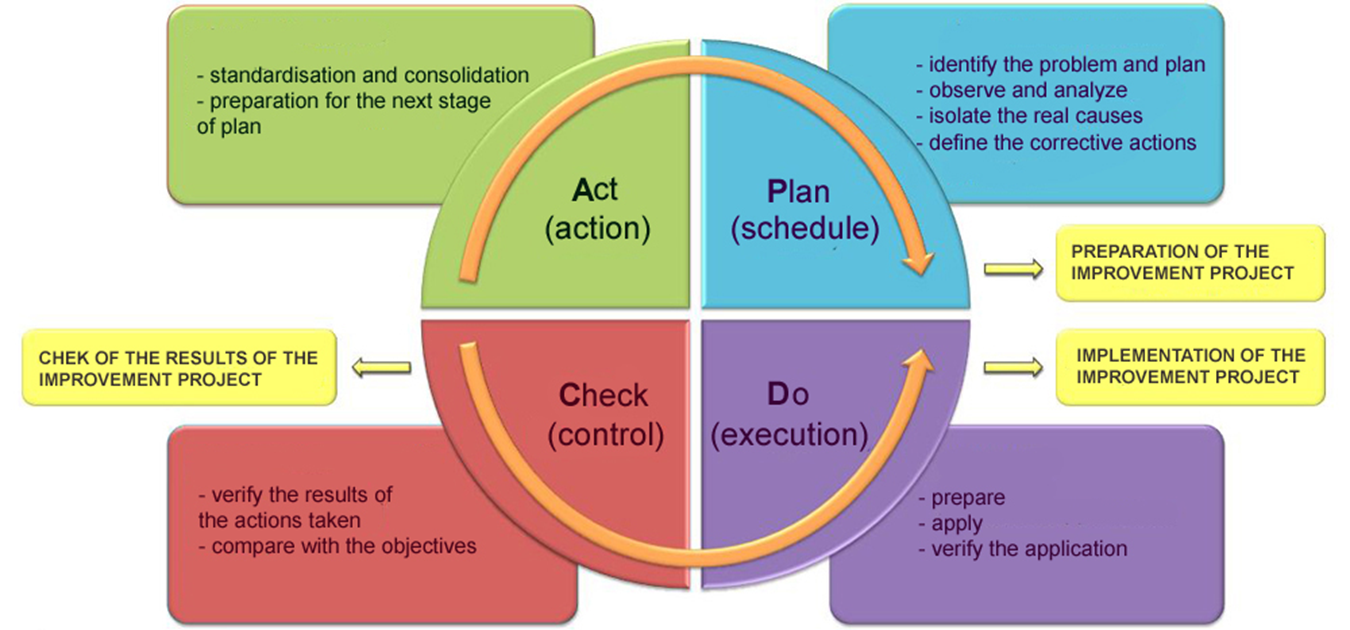
\includegraphics[scale=0.6]{includes/img/pdca.png}
		\caption{Fasi del principio PDCA.}
	\end{figure}
	
	\subsection{Qualità di prodotto}
	Al fine di avere un prodotto di qualità è necessario definire degli obiettivi di qualità e garantire che questi saranno raggiunti. 
	Lo standard ISO/IEC 9126 descrive obiettivi e metriche necessarie a valutarli.
	
	I criteri valutativi sono così suddivisi:
	
	\begin{itemize}
		\item \textbf{Qualità esterna: }le metriche esterne, specificate nella norma ISO/IEC 9126-2, valutano i comportamenti del prodotto sulla base di prove, dell'operatività e dell'osservazione durante la sua esecuzione, in funzione degli obiettivi stabiliti;
		\item \textbf{Qualità interna: }è specificata nella norma ISO/IEC 9126-3 e si applica al software non eseguibile
		durante la progettazione e la codifica dello stesso, le misure effettuate consentono di prevedere il livello di qualità esterna ed interna, in quanto gli attributi interni influenzano quelli esterni e di uso;
		\item \textbf{Qualità d'uso: }Rappresenta la qualità dal punto di vista dell'utente finale, viene raggiunto quando sono raggiunte la qualità esterna e quella interna, le metriche di valutazione sono fornite nella norma ISO/IEC 9126-4.
	\end{itemize}
	
	
	\subsection{Pianificazione strategica e temporale}
	Al fine di ridurre la propagazione di errori, l’attività di verifica di codice e documentazione dovrà essere sistematica. 
	Come procedura preliminare ad ogni attività, sarà necessario un studio preliminare volto ad evitare errori di natura tecnica o concettuale e conseguentemente alleggerire l’attività di verifica postuma.
	Si ha come obiettivo quello di rispettare e scadenze riportate nel \textsc{PianoDiProgetto 1\_0\_0.pdf}.
	
	
	\subsection{Resposanbilità}
	Il \textit{\RdP}\ ha il compito di:
	\begin{itemize}
		\item Accertarsi che attività e ruoli vengano rispettate, come definite nel \textsc{PianoDiProgetto 1\_0\_0.pdf};
		\item Accertarsi che le attività di verifica vengano eseguite sistematicamente, come descritto nelle \textsc{NormeDiProgetto 1\_0\_0.pdf};
		\item Approvare e sancire la distribuzione di un documento.
	\end{itemize}

	I \textit{\Vers}\ hanno il compito di:
	\begin{itemize}
		\item Effettuare l‘attività di verifica in modo sistematico utilizzando metodi e strumenti descritti nel \textsc{PianoDiQualifica 1\_0\_0.pdf};
		\item Documentare e segnalare ogni errore riscontrato.
	\end{itemize}	
	
	
	\subsection{Risorse}
	Per la corretta riuscita del progetto sono necessarie risorse umane, software e hardware.
	
		\subsubsection{Risorse umane}
		\begin{itemize}
			\item \textit{\RdP};
			\item \textit{\Res};
			\item \textit{\Amm};
			\item \textit{\Ver};
			\item \textit{\Prog};
			\item \textit{\Ana}.
		\end{itemize}
		
		\subsubsection{Risorse software}
		Sono necessari i software utili per
		\begin{itemize}
			\item la gestione di documentazione in \LaTeX;
			\item la creazione di diagrammi UML;
			\item lo sviluppo del codice nei linguaggi di programmazione scelti;
			\item l'automatizzazione e semplificazione delle attività di verifica;
			\item l'analisi statica del codice;
			\item la gestione dei test sul codice.
		\end{itemize}
		
		\subsubsection{Risorse hardware}
		\begin{itemize}
			\item personal computer dotati di tutti i software elencati nel \textsc{PianoDiQualifica 1\_0\_0.pdf} e nelle \textsc{NormeDiProgetto 1\_0\_0.pdf};
			\item luoghi dove effettuare le riunioni sia interne che esterne. In caso di riunioni esterne, potrebbe essere necessaria una connessione ad internet per un collegamento SKype con il cliente.
		\end{itemize}
		
						
	\subsection{Misure e metriche}
		Per conseguire dei risultati concreti, il processo di verifica deve fornire dei dati quantificabili per poter valutare se gli obiettivi sono stati raggiunti o meno. Queste è possibile tramite l’utilizzo di metriche e misure. Considerata la poca esperienza del gruppo, questi valori potrebbero essere inizialmente non molto accurati, ma utilizzando il modello incrementale visto nel \textsc{PianoDiProgetto 1\_0\_0.pdf} si potrà migliorarne la precisione.
		Per ogni metrica sono indicati due range:
		\begin{itemize}
			\item \textbf{Range-accettazione: }rappresenta i valori minimi da raggiungere per il conseguimento degli obiettivi di qualità;
			\item \textbf{Range-ottimale: }rappresenta i valori entro cui dovrebbe collocarsi la misurazione. Non sono vincolanti ma nel caso in cui non si raggiungessero questi valori, sarà necessaria una verifica più accurata e una ulteriore discussione, nella riunione successiva, delle cause di questo scostamento.
		\end{itemize}
	
		\subsubsection{Metriche per i documenti}
		
		\subsubsection{Indice Gulpease }
		L'Indice Gulpease è un indice di leggibilità di un testo tarato sulla lingua italiana. Rispetto ad altri ha il vantaggio di utilizzare la lunghezza delle parole in lettere anziché in sillabe, semplificandone il calcolo automatico.
		L'indice di Gulpease considera due variabili linguistiche: la lunghezza della parola e la lunghezza della frase rispetto al numero delle lettere.
		La formula per il suo calcolo è la seguente:
		
		\[ 80+\frac{300*(numero delle frasi)-10*(numero delle lettere)}{numero delle parole} \]
		
		
		I risultati sono compresi tra 0 e 100, dove il valore "100" indica la leggibilità più alta e "0" la leggibilità più bassa. In generale risulta che testi con un indice:
		\begin{itemize}
			\item inferiore a 80 sono difficili da leggere per chi ha la licenza elementare;
			\item inferiore a 60 sono difficili da leggere per chi ha la licenza media;
			\item inferiore a 40 sono difficili da leggere per chi ha un diploma superiore.
		\end{itemize}
	
		I parametri presi in considerazione saranno:
	
		\begin{itemize}
			\item \textbf{Range-accettazione: }[35/100];
			\item \textbf{Range-ottimale: }[45/100].
		\end{itemize}
	
		\subsubsection{Metriche per i processi}
		Le metriche scelte prendono in considerazione tempi e costi, in modo da poter controllare efficacemente i processi e riuscire ad attenersi a quanto deciso nel Piano di Progetto. 
		Per queste metriche non vengono forniti Range-accetazione e Range-ottimale poiché bisognerà consultare il \textsc{PianoDiProgetto 1\_0\_0.pdf} per fare le dovute considerazioni.
		
		\begin{itemize}
			\item \textbf{PPC (Partial Planned Cost): }indica il costo pianificato per lo svolgimento di un sottoinsieme di attività. Si misura in euro e in ore;
			\item \textbf{PV (Planned Value): }indica il valore che si prevede ottenere dal completamento delle attività pianificate. Per questo progetto tale valore corrisponde alla spesa richiesta per il completamento delle attività. Si misura in euro e in ore;
			\item \textbf{EV (Earned Value): }indica il valore ottenuto tramite le attività completate alla data corrente. Per questo progetto tale valore corrisponde alla spesa richiesta per il completamento delle attività. Si misura in euro e in ore;
			\item \textbf{AC (Actual Cost): }indica il costo effettivamente sostenuto alla data corrente. Si misura in euro e in ore. Aiuta a calcolare altre metriche;
			\item \textbf{BAC (Budget at Completion): }costo previsto per portare a termine il progetto. Si misura in euro e in ore. Mantiene traccia della spesa totale preventivata all'inizio del progetto;
			\item \textbf{ETC (Estimate to Complete): }indica i costi pianificati per portare a termine le attività di progetto rimanenti alla data corrente. Corrisponde al PV riesaminato allo stato corrente del progetto ma senza tenere conto delle attività completate. Si misura in euro e in ore;
			\item \textbf{EAC (Estimated at Completion): }revisione del costo stimato per la realizzazione del progetto, ossia il BAC rivisto allo stato corrente del progetto. Si misura in euro e in ore e si ottiene dalla formula: EAC = AC + ETC;
			\item \textbf{SV (Schedule Variance): }è un indicatore di efficacia, mostra se si è o meno in linea con la pianificazione temporale rispetto alle attività nella baseline. Una schedule variance positiva indica che il gruppo è in anticipo rispetto al Piano di progetto, altrimenti è in ritardo. Si ottiene dalla formula: SV = EV - PV;
			\item \textbf{BV (Budget Variance): }indica se la spesa sostenuta alla data corrente è superiore o inferiore a quella preventivata. Una budget variance positiva indica che si è speso meno di quanto inizialmente previsto,  altrimenti viceversa. Si ottiene dalla formula: BV = PV - AC.
			
		\end{itemize}
		
		
		\subsubsection{Metriche per il codice}
		Le metriche per il software ora descritte non sono definitive, ma saranno affinate successivamente.
		
		\begin{itemize}
			\item \textbf{Attributi per classe: }un grande numero di attributi interni ad una classe mostra probabilmente la necessità di suddividere la classe in più classi relazionate tra loro.
			
			\begin{itemize}
				\item \textbf{Range-accettazione: }[0/18];
				\item \textbf{Range-ottimale: }[2/9].
			\end{itemize}
		
			\item \textbf{Numero livelli annidamento: }mostra il livello di annidamento dei metodi. Un numero alto implica una bassa astrazione del codice ed un' elevata complessità.
			
			\begin{itemize}
				\item \textbf{Range-accettazione: }[1/8];
				\item \textbf{Range-ottimale: }[1/4].
			\end{itemize}
			
			\item \textbf{Numero parametri per metodo: }un valore elevato indica che probabilmente il metodo ha un sovraccarico di funzionalità.
			
			\begin{itemize}
				\item \textbf{Range-accettazione: }[0/8];
				\item \textbf{Range-ottimale: }[0/5].
			\end{itemize}
			
			\item \textbf{Accoppiamento afferente: }indica il numero di classi esterne ad un package che dipendono da esso. Un grande valore indica una forte dipendenza del software per il package in questione, un valore basso invece indica una bassa utilità del package per il resto del software.
			
			\begin{itemize}
				\item \textbf{Range-accettazione: }non ancora definito;
				\item \textbf{Range-ottimale: }non ancora definito.
			\end{itemize}
			
			\item \textbf{Accoppiamento efferente: }il numero di classi di un package che dipendono da package esterni. Un valore basso indica che il package ha numerose funzionalità indipendenti dal resto del software.
			
			\begin{itemize}
				\item \textbf{Range-accettazione: }non ancora definito;
				\item \textbf{Range-ottimale: }non ancora definito.
			\end{itemize}
			
			\item \textbf{Source Line Of Code (SLOC): }il numero di istruzioni presenti nel codice. Questa metrica fornisce una stima della complessità del programma. È utile anche per dare una stima di quanto il codice incrementerà nel tempo, semplificando così la pianificazione.
			
			\begin{itemize}
				\item \textbf{Range-accettazione: }[0/18];
				\item \textbf{Range-ottimale: }[2/9].
			\end{itemize}
			
			\item \textbf{Complessità Ciclomatica: }una metrica sviluppata da Thomas J. McCabe che consente di stimare la complessità di un programma misurando il numero di cammini linearmente indipendenti attraverso il grafo di controllo di flusso.
			
			\begin{itemize}
				\item \textbf{Range-accettazione: }non ancora definito;
				\item \textbf{Range-ottimale: }non ancora definito.
			\end{itemize}
			
			
		
		\end{itemize}
		
		
	\subsection{Analisi}
	
		\subsubsection{Analisi statica}
		L'analisi statica non necessita dell'esecuzione del codice oggetto ed è applicabile sin da subito su codice e documenti prodotti. Essa ha lo scopo di trovare anomalie e può essere eseguita nei due modi seguenti.
		
		\subsubsection{Walkthrough}
		Questa tecnica consistente nella ricerca a largo spettro di qualsiasi tipo di errore, nel modo più generico possibile. 
		Questa tecnica è utilizzata nelle prime fasi di verifica. Durante ogni fase di verifica verrà stilata una lista degli errori più frequenti, in modo da facilitare l’individuazione delle anomalie nelle fasi successive. 
		Nel momento in cui si avrà a disposizione una lista sufficientemente dettagliata, si potrà passare al metodo Inspection.
		
		
		\subsubsection{Inspection}
		Questo metodo si basa sulla lista prodotta precedentemente con il metodo Walkthrough. In questo modo si andrà a cercare in modo mirato gli errori già individuati in passato, prestando comunque attenzione a nuovi possibili errori, che andranno poi ad arricchire la lista
		
		
		\subsubsection{Analisi dinamica}
		Da definire
		
		
	
\newpage
\section{Resoconto delle attività di verifica}

	\subsection{Dettaglio delle verifiche tramite analisi}
	
	\subsubsection{Documenti}
	
	\paragraph{Fase di Analisi}
	
	



\end{document}